% Template for Cogsci submission with R Markdown

% Stuff changed from original Markdown PLOS Template
\documentclass[10pt, letterpaper]{article}

\usepackage{cogsci}
\usepackage{pslatex}
\usepackage{float}
\usepackage{caption}

% amsmath package, useful for mathematical formulas
\usepackage{amsmath}

% amssymb package, useful for mathematical symbols
\usepackage{amssymb}

% hyperref package, useful for hyperlinks
\usepackage{hyperref}

% graphicx package, useful for including eps and pdf graphics
% include graphics with the command \includegraphics
\usepackage{graphicx}

% Sweave(-like)
\usepackage{fancyvrb}
\DefineVerbatimEnvironment{Sinput}{Verbatim}{fontshape=sl}
\DefineVerbatimEnvironment{Soutput}{Verbatim}{}
\DefineVerbatimEnvironment{Scode}{Verbatim}{fontshape=sl}
\newenvironment{Schunk}{}{}
\DefineVerbatimEnvironment{Code}{Verbatim}{}
\DefineVerbatimEnvironment{CodeInput}{Verbatim}{fontshape=sl}
\DefineVerbatimEnvironment{CodeOutput}{Verbatim}{}
\newenvironment{CodeChunk}{}{}

% cite package, to clean up citations in the main text. Do not remove.
\usepackage{apacite}

% KM added 1/4/18 to allow control of blind submission


\usepackage{color}

% Use doublespacing - comment out for single spacing
%\usepackage{setspace}
%\doublespacing


% % Text layout
% \topmargin 0.0cm
% \oddsidemargin 0.5cm
% \evensidemargin 0.5cm
% \textwidth 16cm
% \textheight 21cm

\title{Consistency and variability in two children's home visual environment
across development}


\author{{\large \bf Morton Ann Gernsbacher (MAG@Macc.Wisc.Edu)} \\ Department of Psychology, 1202 W. Johnson Street \\ Madison, WI 53706 USA \AND {\large \bf Sharon J.~Derry (SDJ@Macc.Wisc.Edu)} \\ Department of Educational Psychology, 1025 W. Johnson Street \\ Madison, WI 53706 USA}

\begin{document}

\maketitle

\begin{abstract}
Include no author information in the initial submission, to facilitate
blind review. The abstract should be one paragraph, indented 1/8 inch on
both sides, in 9\textasciitilde{}point font with single spacing. The
heading `Abstract' should be 10\textasciitilde{}point, bold, centered,
with one line of space below it. This one-paragraph abstract section is
required only for standard six page proceedings papers. Following the
abstract should be a blank line, followed by the header `Keywords' and a
list of descriptive keywords separated by semicolons, all in
9\textasciitilde{}point font, as shown below.

\textbf{Keywords:}
Add your choice of indexing terms or keywords; kindly use a semi-colon;
between each term.
\end{abstract}

\section{Introduction}\label{introduction}

What do children tend to see in their everyday lives? While an
understanding of children's visual environment is central to both
theories of language acquisition and visual development, we know
remarkably little about the categories and objects that tend to be in
the infant view, or how they are experienced. For example, how often do
infants tend to see animals in real-life vs.~in storybooks or as toys?
How consistent are the broad characteristics of children's visual
environment across individuals and across developmental time?

Over the past decade, researchers have begun to answer these questions
by documenting the infant egocentric perspective using head-mounted
cameras (Franchak, Kretch, Soska, \& Adolph, 2011; Yoshida \& Smith,
2008),quantifying the degree to which there are substantial shifts in
infants viewpoints that may have downstream developmental
consequences.\\
Indeed, as adults it is hard to intuit how strange this viewpoint can
be, and how much it varies across development, transitioning over the
first two years of life from close-up views of faces to restricted views
of hands manipulating objects ({\textbf{???}}; Fausey, Jayaraman, \&
Smith, 2016) and children's postural developments shaping what they see
({\textbf{???}}). Most work, however, has focused on documenting the
social information that infants and children have access to across early
development ({\textbf{???}}; Fausey et al., 2016; Yoshida \& Smith,
2008).

More recent research has made progress towards understanding what
objects tend to be the infant view, starting with annotating the
basic-level categories (e.g., spoons, cups) in the view of 8-month-olds
during mealtime. This research suggests that a small number of objects
are both pervasively present and among infants' first-learned words
(Clerkin, Hart, Rehg, Yu, \& Smith, 2017), pointing towards a link
between visual experience and early word learning. These findings
suggest that a more complete understanding of the visual environment of
infants and young children could yield insights about the inputs to both
category learning and word learning.

Here, we take a step towards characterizing the visual environment of
young children by analyzing the categories of objects (e.g., animals,
vehicles, toys, people) present in the infant view in a longitudinal
corpus of head-mounted camera data ({\textbf{???}}). We choose to
annotate these broad categories -- rather than the basic-level
identities of objects -- for three reasons. First, as our corpus is
sampled densely from only a few children, an understanding of the
particular objects in their viewpoints may not be particularly
generalizable. Second, the basic-level identities of many objects --
especially certain toys or objects viewed from odd angles -- are
sometimes ambiguous (and therefore would be inconsistent across
annotators). Finally, these less detailed annotations allow us to
collect annotations for more frames from the dataset and therefore
license broader coverage. We thus collected human annotations of a
randomly sampled set of 24,000 frames from two children in the
longitudinal dataset, allowing the analysis of the proportion of broad
categories in the infant view from 6-32 months of age.

Using these annotations, we conducted three sets of analyses. First, we
examined whether the proportion of animals vs.~inanimate objects would
be relatively equal in the infant view. A long literature has documented
that even newborns have a tendency to attend to animate agents
({\textbf{???}}), and visual cortex dedicates a remarkable amount of
space to making fine-grained distinctions among different animals
({\textbf{???}}). Furthermore, animal words tend to be among children's
first-learned words (CITES). However, at present, it is unknown whether
(non-human) animates (e.g., cats, dogs, other animals) are prevalent in
the infant viewpoint, and whether they tend to be exemplars of real-life
animals (e.g., ducks at a park, pet dogs) or mostly illustrations in
storybooks or as toy stuffed animals.

Second, we examined the co-occurrence between these broad object
categories across visual scenes. While some activity contexts (e.g.,
storytime) and lead to intuitive co-occurrences between object
categories (e.g., between books and people), not all activities are
intuitive or consistent. We conducted a set of data-driven, exploratory
analyses of the co-occurrence statistics of these broad categories to
identify other, reliable patterns in how infants experience their visual
world.

Finally, prior work documenting the proportion of faces/hands in view
has suggested some developmental changes in how children experience
their visual across this same age range--including in this same dataset
({\textbf{???}}). Thus, one possibility is that as children learn to
crawl and walk on their own ({\textbf{???}}, {\textbf{???}}; Franchak et
al., 2011), some categories that children are likely to interact with
(i.e., toys, small objects) could become more prevalent in the child's
view across age, whereas other, more stable categories (i.e., furniture)
might show relative consistency. On the other hand, the broad
characteristics children's visual environments may be relatively stable
and determined mostly by the activities that they tend to engage in. We
thus examined this hypothesis by exploring the prevalence of each of the
broad categories that were annotated across developmental time and
across both children.

\section{Method}\label{method}

\subsection{Dataset}\label{dataset}

\subsection{Annotation procedure}\label{annotation-procedure}

\subsection{Preprocessing}\label{preprocessing}

\section{Results}\label{results}

\subsection{Part 1: Category
prevalence}\label{part-1-category-prevalence}

Lots of people generally speaking (and partial views of furniture) Equal
proportion of toys vs.~real for animals/vehicle Not that much variance
in exemplars for reals -- mostly dog/cats for animals Real vehicles are
often interiors of vehicles (can quantify how many easily) Animacy/size
prevalence comparisons More objects \textgreater{} animals in general
Even though animal names are learned early Suggests role for heightened
attention to animals Small objects → broad category of stuff they see
Some of this measured in mealtime, but a lot more variability here than
just food/utensils (toys/other small objects, etc) No developmental
change in prevalence AFAWCT (maybe in stereotyped activities, not done
yet) Is there a dip for toys? (less play as learning locomotion?)

\begin{CodeChunk}
\begin{figure*}[h]

{\centering 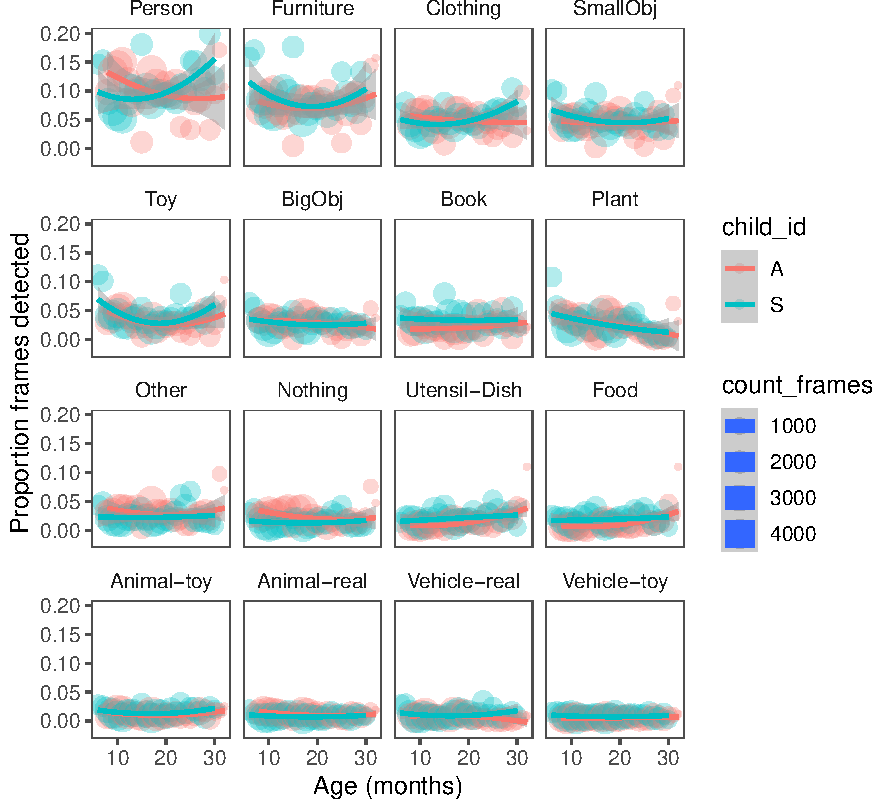
\includegraphics{figs/freq_by_category-1} 

}

\caption[Frequency of categories annotated across the 24K random frames plotted as a function of each child's age (in months)]{Frequency of categories annotated across the 24K random frames plotted as a function of each child's age (in months).}\label{fig:freq_by_category}
\end{figure*}
\end{CodeChunk}

\begin{CodeChunk}
\begin{figure}[h]

{\centering 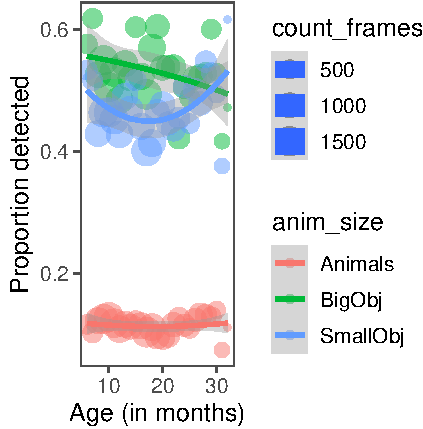
\includegraphics{figs/anim_size-1} 

}

\caption[Frequency of animals (including toys) relative to big and small inaniamte objects detected in the dataset]{Frequency of animals (including toys) relative to big and small inaniamte objects detected in the dataset.}\label{fig:anim_size}
\end{figure}
\end{CodeChunk}

\subsection{Part 2: Co-occurrence of categories in visual
scenes}\label{part-2-co-occurrence-of-categories-in-visual-scenes}

Stereotyped activities with/without parent Separation of these
activities by child-alone vs.~with parent (adult-hand or adult-face
present) Mealtime (food + utensil?) Storytime (book + person) or book on
own Joint playtime (not book + yes toy + person) Data-driven:
Correlogram of different categories (and hierarchical clustering to
identify similar/dissimilar contexts) Might identify the candidate
contexts that we can think of, and maybe others that we can't (e.g.,
perhaps playtime outside)

\begin{CodeChunk}
\begin{figure*}[h]

{\centering 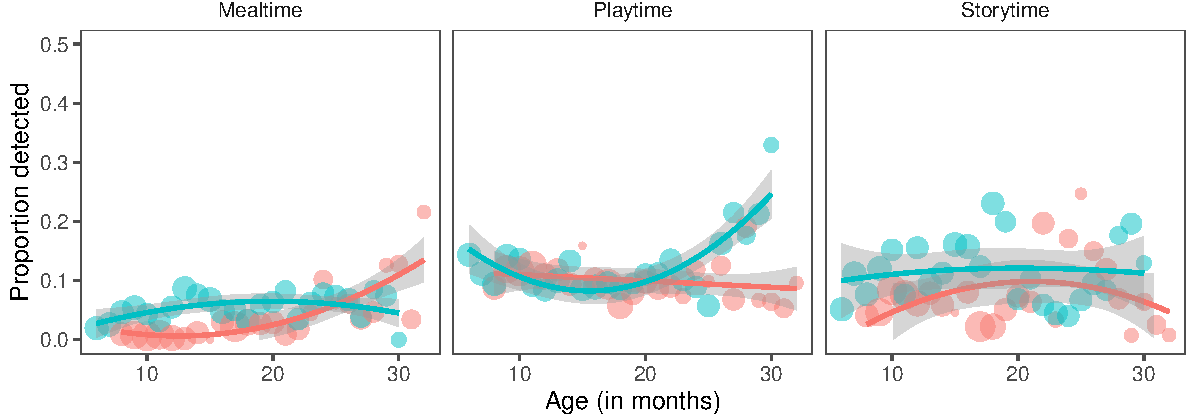
\includegraphics{figs/activities-1} 

}

\caption[Frequency of mealtime (food = utensils), storytime (book + person), and playtime (e.g., toy + people) activities for each child across age in the randomly sampled frames]{Frequency of mealtime (food = utensils), storytime (book + person), and playtime (e.g., toy + people) activities for each child across age in the randomly sampled frames. }\label{fig:activities}
\end{figure*}
\end{CodeChunk}

\begin{CodeChunk}
\begin{figure}[h]

{\centering 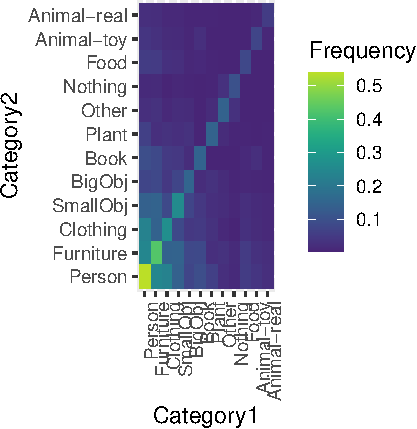
\includegraphics{figs/coocc_stats-1} 

}

\caption[Co-ccurance between different categories detected in the dataset across all frames]{Co-ccurance between different categories detected in the dataset across all frames. }\label{fig:coocc_stats}
\end{figure}
\end{CodeChunk}

\section{General Discussion}\label{general-discussion}

Discussion Main findings Relative consistency in the visual environment
over age, posture/other changes may be having more fine-grained impacts
on HOW children see objects (and the diversity at the basic-level)
Stereotyped activities are not that frequent in kid's experience, even
though we think of them often (and this is parents putting headcam's on
their kids, so maybe they are even overrepresented relative to normal)
Kids learning from both real and toy examples in equal measure →
toys/depictions are real part of kid's representations Role of extra
attention to animals (i.e.~saliency of animate objs) in learning
animals/their names, not just pure frequency

Future work Relationship to early learned words for these categories →
need to drill down to basic-level categories to assess this hypothesis
Generalization to other datasets Fine-tuning/training of models to do so
and make broader conclusions

Limitations WEIRD kids who have a lot of books and toys and may not go
outside as much → may really vary across kids, SES, contexts, etc Yet
suggests that at least some kids are learning quite a lot from books and
depictions Only 2 kids -- though we see consistency here When parents
choose to wear headcam -- not getting time at daycare,etc Nonetheless,
broad findings that objects \textgreater{} animals and consistency
across age are things we predict will generalize broadly beyond this
small population

\section{Acknowledgements}\label{acknowledgements}

Place acknowledgments (including funding information) in a section at
the end of the paper.

\section{References}\label{references}

\setlength{\parindent}{-0.1in} \setlength{\leftskip}{0.125in} \noindent

\hypertarget{refs}{}
\hypertarget{ref-clerkin2017}{}
Clerkin, E. M., Hart, E., Rehg, J. M., Yu, C., \& Smith, L. (2017).
Real-world visual statistics and infants' first-learned object names.
\emph{Phil. Trans. R. Soc. B}, \emph{372}(1711), 20160055.

\hypertarget{ref-fausey2016}{}
Fausey, C. M., Jayaraman, S., \& Smith, L. (2016). From faces to hands:
Changing visual input in the first two years. \emph{Cognition},
\emph{152}, 101--107.

\hypertarget{ref-franchak2011}{}
Franchak, J. M., Kretch, K. S., Soska, K. C., \& Adolph, K. E. (2011).
Head-mounted eye tracking: A new method to describe infant looking.
\emph{Child Development}, \emph{82}(6), 1738--1750.

\hypertarget{ref-yoshida2008}{}
Yoshida, H., \& Smith, L. (2008). What's in view for toddlers? Using a
head camera to study visual experience. \emph{Infancy}, \emph{13},
229--248.

\bibliographystyle{apacite}


\end{document}
